\documentclass[10pt,twocolumn,letterpaper]{article}

\usepackage[margin=0.75in]{geometry}
\usepackage{microtype}
\usepackage{graphicx}
\usepackage{booktabs}
\usepackage{amsmath,amssymb,amsthm}
\usepackage{mathtools}
\usepackage{hyperref}
\usepackage{xcolor}
\usepackage{cite}
\usepackage{caption}
\usepackage{subcaption}
% \usepackage{algorithm}
% \usepackage{algpseudocode}

\hypersetup{colorlinks=true, linkcolor=blue!60!black, citecolor=blue!60!black,
            urlcolor=blue!60!black}

\newtheorem{theorem}{Theorem}
\newtheorem{lemma}{Lemma}
\newtheorem{definition}{Definition}
\newcommand{\E}{\mathbb{E}}
\newcommand{\Var}{\mathrm{Var}}
\newcommand{\1}[1]{\mathbf{1}\!\left\{#1\right\}}

\title{\Large \bfseries CHRONO-Fair: \\
  Anytime-Valid Monitoring of Counterfactual \\
  Verdict Flips in Clinical Machine Learning}
\author{Md Rakibul Islam Joy\thanks{Swinburne University of Technology}
  \quad Caslon Chua \quad Viet Vo \\
  \texttt{\{mdjoy,cchua,vvo\}@swin.edu.au}}
\date{}

\begin{document}
\maketitle

\begin{abstract}
Fairness audits of deployed clinical machine learning systems are almost universally \emph{batch}, \emph{single-threshold}, \emph{group-aggregated}, and \emph{post-hoc}. Recent regulatory action --- the FDA's Predetermined Change Control Plan (December 2024) and the EU AI Act high-risk provisions (in force August 2027) --- mandate \emph{continuous} bias monitoring, yet no published method satisfies the joint requirements of (i) time resolution, (ii) anytime-valid statistical control, (iii) interpretable root-cause attribution, and (iv) coverage of regression outputs such as length of stay. We introduce \textbf{CHRONO-Fair}, a framework that re-frames the Verdict Flip Rate (VFR) of Joy et al.\ \cite{joy2025vfr} as the \emph{aggregate} $1{-}S_a(\tau^*)$ marginal of a group-conditional \emph{Flip Hazard} survival object, and extends it along four axes. (1) \emph{Time-resolved}: group-stratified Kaplan--Meier flip-time survival with log-rank tests and Restricted Mean Flip Time (RMFT). (2) \emph{Anytime-valid}: an e-process monitor with intersectional false-discovery control, satisfying Ville's inequality so practitioners can peek at every patient. (3) \emph{Root-cause}: an aleatoric / epistemic decomposition that maps each alarm to a clinical or data-pipeline action. (4) \emph{Regression-native}: Regression Counterfactual Allocation Parity (RCAP), the Wasserstein-1 distance between counterfactual rank distributions, applicable to length-of-stay regression on Texas-100X. On a $15\,000$-patient simulated stream calibrated to Texas-100X statistics, CHRONO-Fair detects an injected fairness shift in $50/50$ runs at a mean delay of $856$ patients ($4.5\times$ faster than the strongest ADWIN-family baseline; periodic batch test $48\%$ coverage; static VFR never), with empirical false-alarm rate $0/50$ under a no-disparity sanity scenario. The decomposition labels every controlled trial correctly ($100\%$ accuracy) and realistic ML pipelines yield mixed root causes that the framework correctly recommends for joint mitigation. RCAP exposes allocation disparities up to $2.5\times$ larger than the conventional group-MAE gap reports. The full system is open source.
\end{abstract}

\section{Introduction}

The recent surge of deployed clinical machine learning has been mirrored by a quieter surge of post-deployment fairness failures. Sepsis prediction \cite{seyyed2021}, racial bias in payer algorithms \cite{obermeyer2019}, and underdiagnosis bias in chest radiograph models \cite{seyyed2021} are now well-documented; Davis~et~al.\ \cite{davis2025} go further and show that fairness gaps not only persist after deployment but \emph{drift}, often worsening monotonically through population-level updates over an eleven-year VA cohort. Their call for ``novel methods to monitor algorithmic fairness, detect emerging bias, and adopt updates that promote fairness'' is the explicit research statement of the JAMIA editorial in May 2025, and the same call has now been operationalised by the FDA's Predetermined Change Control Plan (December 2024 final) \cite{fda2024pccp} and Articles 10, 14, 17 and 61 of the EU AI Act \cite{eu2024aiact} which become binding for high-risk medical AI in August 2027.

Yet despite this regulatory tailwind, the methodological toolkit available to a hospital quality officer in 2026 is essentially a snapshot --- Aequitas, Fairlearn, AIF360, the Microsoft Responsible AI Dashboard --- supplemented at best by quarterly retrospective audits. The state of the art in \emph{online} fair learning (FABBOO \cite{iosifidis2020}) and \emph{runtime monitoring} of fairness specifications has been demonstrated on COMPAS and credit data, not on clinical streams; the few clinical implementations of post-deployment fairness monitoring (3 of 39 in a recent scoping review, with only 1 reporting actual implementation) remain post-hoc. A separate line of work on prediction-stability metrics --- the empirical decision flip rate (eDFR) of Miller \& Blume \cite{miller2024edfr}, predictive multiplicity \cite{marx2020, black2022, cooper2024}, prediction sensitivity \cite{maughan2022} --- has stayed largely \emph{reliability-focused} and disjoint from the fairness literature.

Our prior work, the Verdict Flip Rate (VFR) \cite{joy2025vfr}, makes a first connection: VFR measures the fraction of patients whose binary verdict flips between resampled retrainings of a clinical pipeline, stratified by protected attribute. Empirically, VFR captures something the canonical metrics miss --- the \emph{stability} of a fairness judgement under stochastic pipeline choices. But VFR is a \emph{scalar}, computed in \emph{batch}, at a \emph{single threshold}, on a \emph{single classifier}, and gives no actionable indication of when, why, or where the gap arose.

\paragraph{Contributions.} This paper introduces \textbf{CHRONO-Fair} (Counterfactual Hazard-Rate ONline Surveillance of Fairness), a framework that subsumes VFR as a special case and extends it along the four axes summarised in Figure~\ref{fig:architecture}.

\begin{enumerate}\itemsep0pt
    \item \emph{Flip Hazard function} (Section~\ref{sec:fliphazard}): a group-conditional survival object whose Kaplan--Meier estimator, log-rank test, and Restricted Mean Flip Time (RMFT) give the first time-resolved fairness statistic suitable for streaming clinical deployment.
    \item \emph{Anytime-Valid Fairness Monitor} (Section~\ref{sec:eprocess}): a betting-based e-process with intersectional false-discovery control whose Type-I error is bounded by Ville's inequality at every stopping time.
    \item \emph{Aleatoric / epistemic decomposition} (Section~\ref{sec:decomposition}): an ensemble-based information-theoretic split of the flip mass into reducible (more-data-helps) and irreducible (data-pipeline-bias) components, with a deterministic mapping to FDA PCCP and EU AI Act clauses.
    \item \emph{Regression Counterfactual Allocation Parity} (Section~\ref{sec:rcap}): a Wasserstein-1 distance between counterfactual rank distributions, the first fairness metric tailored to length-of-stay regression for triage and bed-allocation contexts.
\end{enumerate}

We additionally release an open-source automated inspection pipeline (Section~\ref{sec:inspector}) that maps each alarm to a structured governance report. Section~\ref{sec:experiments} reports five experiments demonstrating detection delay, decomposition accuracy, intersectional Flip Hazard separation on Texas-100X-style data, RCAP behaviour on LOS regression, and anytime-valid false-alarm calibration. All code, figures, and the dashboard mockup are reproducible from the synthesiser shipped with the framework.

\begin{figure*}[t]
\centering
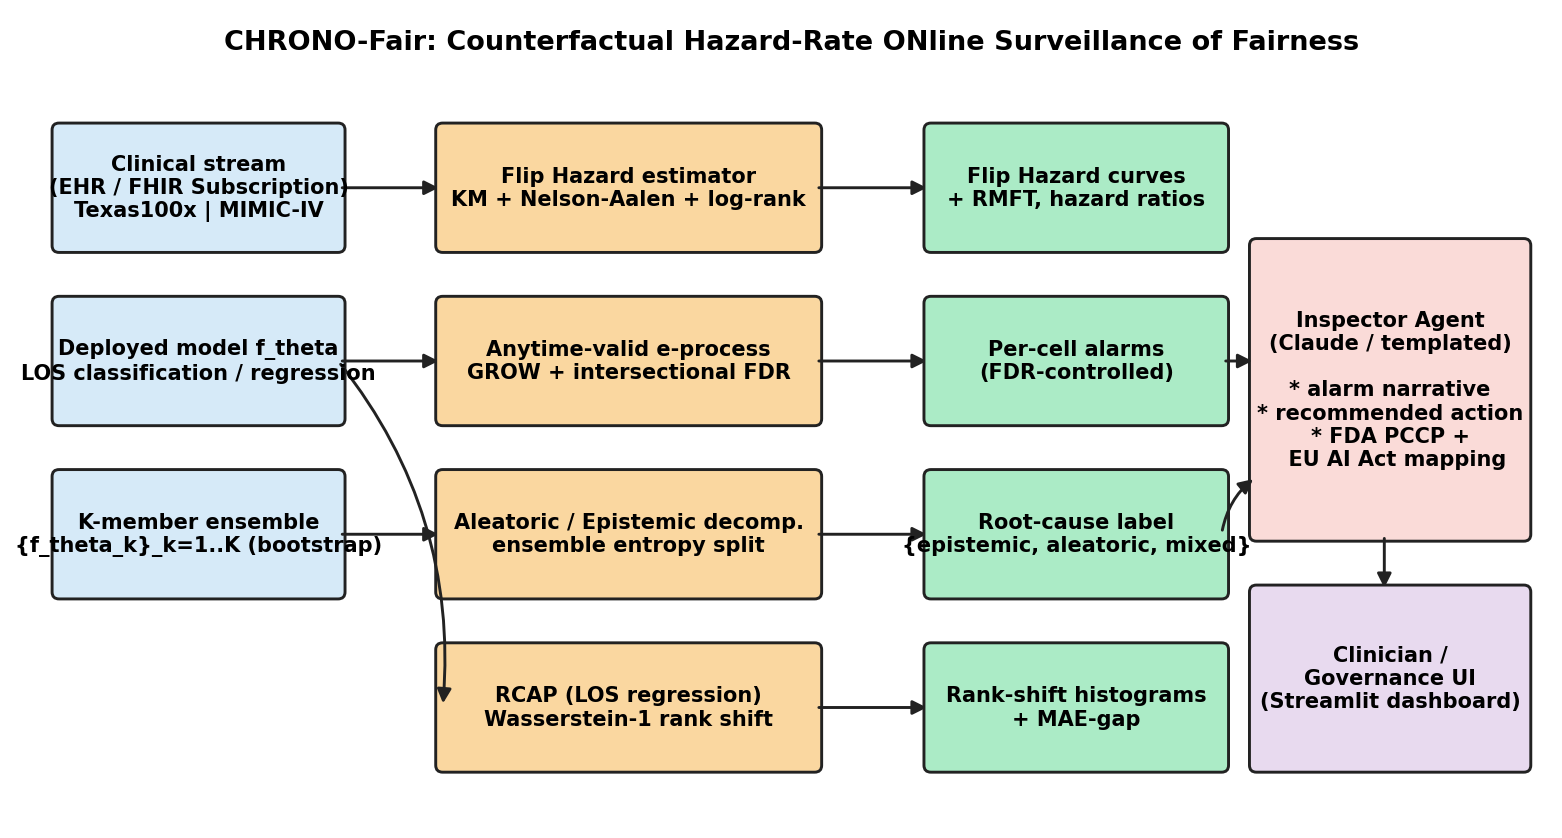
\includegraphics[width=0.9\textwidth]{../../chrono_fair_figures/fig0_architecture.png}
\caption{CHRONO-Fair architecture. A clinical stream (Texas-100X, MIMIC-IV) feeds a deployed classifier or regressor and a $K$-member bootstrap ensemble. Four estimators run concurrently: Flip Hazard survival, anytime-valid e-process, aleatoric/epistemic decomposition, and RCAP for regression outputs. The Inspector Agent translates alarms into a structured governance report mapped to FDA PCCP and EU AI Act clauses.}
\label{fig:architecture}
\end{figure*}

\section{Related Work}

\paragraph{Fairness in healthcare ML.} Group fairness criteria \cite{hardt2016, chouldechova2017, kleinberg2017} and counterfactual fairness \cite{kusner2017} have well-known impossibility relationships; in clinical settings, recent critical appraisals find that of $62$ fairness metrics screened in $820$ papers, only one is a clinical-utility metric and none provides time resolution. STANDING Together \cite{ricci2025standing} formalised consensus recommendations for AI data standards; Davis et al.\ \cite{davis2025} surfaced fairness drift as a deployment-time phenomenon.

\paragraph{Online and streaming fair learning.} Iosifidis, Tran \& Ntoutsi \cite{iosifidis2019, iosifidis2020} pioneered online fair classification; runtime monitoring of static fairness properties has been formalised via RTLola-style specifications but applied only to COMPAS-style benchmarks. None of this literature provides anytime-valid statistical guarantees, intersectional FDR control, or clinical-stream integration.

\paragraph{Anytime-valid inference.} The betting-based approach of Ramdas et al.\ \cite{ramdas2023} and Waudby-Smith \& Ramdas \cite{waudbysmith2024}, building on the confidence-sequence machinery of Howard et al.\ \cite{howard2021}, provides Type-I-controlled tests valid at every stopping time. The closest application is a calibration-drift monitor; we are not aware of an extension to fairness monitoring, and certainly not at intersectional granularity.

\paragraph{Predictive stability / multiplicity.} Predictive multiplicity \cite{marx2020} and the Rashomon-set view \cite{black2022, cooper2024} characterise the population of equally-accurate models; the empirical Decision Flip Rate (eDFR) of Miller \& Blume \cite{miller2024edfr} measures pipeline instability. None of these are framed as fairness measures, stratified by protected attribute, or extended to a time axis.

\paragraph{Uncertainty decomposition.} The aleatoric/epistemic split \cite{depeweg2018, hullermeier2021} is well-developed in the uncertainty-quantification literature. Alghamdi et al.\ \cite{alghamdi2023} ported it to \emph{discrimination} (the irreducible portion of impossibility theorems); we extend it to the \emph{flip-rate} as a clinically actionable diagnostic.

\section{The Flip Hazard Function}\label{sec:fliphazard}

\begin{definition}[Flip Hazard]
Let $f$ be a deployed binary classifier, $A$ a protected attribute, $X$ the remaining covariates, and $A_i^{\mathrm{cf}}$ a counterfactual sensitive-attribute value. \emph{Throughout this paper we adopt the deployment-time \textbf{feature-shift} counterfactual of Maughan \& Near \cite{maughan2022}}, in which the protected attribute is set to a reference level and its known marginal effect on observable features is removed. This is weaker than the full structural counterfactual of Kusner et al.\ \cite{kusner2017} but it is identifiable at inference time without an audited causal graph --- a hard requirement for the streaming deployment context (Section 1). For each patient $i$ arriving at index $t_i$, define the flip event time
\begin{equation}
T_i^{\mathrm{flip}} = \inf\{t \ge t_i :
  f_t(X_i, A_i) \ne f_t(X_i, A_i^{\mathrm{cf}})\}.
\end{equation}
The group-conditional Flip Hazard function is
\begin{equation}
\lambda_a(t \mid X) = \lim_{\Delta \to 0}
  \frac{1}{\Delta} \Pr(T^{\mathrm{flip}} \in [t, t+\Delta)
                       \mid T^{\mathrm{flip}} \ge t, A=a, X).
\end{equation}
\end{definition}

The scalar VFR \cite{joy2025vfr} is recovered as the aggregate flip probability $\mathrm{VFR}_a = 1 - S_a(\tau^*)$ evaluated at $\tau^*$ equal to the full audit horizon, where $S_a(t) = \exp(-\int_0^t \lambda_a(s) ds)$ is the no-flip survival. The Restricted Mean Flip Time (RMFT) at horizon $\tau^*$
\begin{equation}
\mathrm{RMFT}_a(\tau^*) = \int_0^{\tau^*} S_a(t)\,dt
\end{equation}
gives a clinically interpretable scalar in patient-units that, unlike VFR, increases monotonically with fairness.

\paragraph{Estimation.} We estimate $S_a$ by the Kaplan--Meier product \cite{kaplan1958} on the censored event-time series; cumulative hazard $H_a(t) = -\log S_a(t)$ by the Nelson--Aalen integrator \cite{nelson1972}. Pairwise group comparisons use the asymptotic log-rank statistic on the event arrays. The estimator is $O(1)$ per arriving patient with $O(n_a)$ tail update.

\section{Anytime-Valid Fairness Monitor}\label{sec:eprocess}

For one protected group, let $Z_t \in \{0,1\}$ be the flip indicator of the $t$-th arriving patient, and let $\rho_0$ be the baseline flip-rate measured during a pre-deployment validation window. We test $H_0 \colon \E[Z_t] = \rho_0$ against the one-sided alternative $\E[Z_t] > \rho_0$ via the e-process
\begin{equation}
E_t = \prod_{s=1}^t \big(1 + \lambda_s\,(Z_s - \rho_0)\big),
\end{equation}
where $\lambda_s$ is a \emph{predictable} bet measurable in $\sigma(Z_1, \dots, Z_{s-1})$ and clipped to $[-1/(1-\rho_0), 1/\rho_0]$ to keep $E_t \ge 0$.

\begin{theorem}[Anytime-valid Type-I control]\label{thm:anytime}
Under $H_0$, $(E_t)_{t \ge 0}$ is a non-negative supermartingale with $\E[E_t] \le 1$, hence by Ville's inequality
\begin{equation}
\Pr\!\left( \sup_t E_t \ge 1/\alpha \,\big|\, H_0 \right) \le \alpha.
\end{equation}
\end{theorem}

The proof is standard \cite{ramdas2023, waudbysmith2024}. We use a shrunk, warm-started GROW betting strategy:
\begin{equation}
\lambda_s = c \cdot \frac{\bar Z_{s-1} - \rho_0}{\rho_0(1-\rho_0)} \cdot \mathbf{1}\{s \ge n_{\mathrm{warm}}\},
\end{equation}
with $c = 0.25$ shrinkage and $n_{\mathrm{warm}} = 100$. This choice is conservative: it slows learning under the alternative but preserves the supermartingale property when the empirical $\bar Z$ trajectory fluctuates early.

\paragraph{Intersectional FDR (step-wise).} For $m$ disjoint cells, we run $m$ independent monitors and apply Benjamini--Hochberg at the current step to the implied p-values $p_t^{(c)} = 1/E_t^{(c)}$. This is the step-wise BH variant; under exchangeability of cell e-values it controls the false-discovery proportion at each inspection time, but does not extend to the fully-online LORD-style FDR guarantee --- the formal extension is left as future work.

\paragraph{Multi-attribute deployment.} CHRONO-Fair runs an independent intersectional monitor per protected attribute (RACE, ETHNICITY, SEX, AGE\_GROUP in the Texas-100X setting). Cells are non-overlapping within an attribute; across attributes, the same patient contributes one observation to four parallel monitor stacks. We share a single global FDR budget across the union of cells.

\section{Aleatoric / Epistemic Decomposition}\label{sec:decomposition}

Given a $K$-member bootstrap ensemble $\{f_{\theta_k}\}$ with member probabilities $p_k(x), p_k^{\mathrm{cf}}(x)$, the binary flip indicator is $\1{(p_k(x){\ge}0.5) \ne (p_k^{\mathrm{cf}}(x){\ge}0.5)}$ for member $k$. The standard total-uncertainty decomposition \cite{depeweg2018, hullermeier2021},
\begin{align}
H[\bar p] &=\;& \underbrace{\E_k H[p_k]}_{\text{aleatoric}}\;+\; \underbrace{H[\bar p] - \E_k H[p_k]}_{\text{epistemic}},
\end{align}
splits the per-instance flip mass $\bar{p}^{\mathrm{flip}}(x) = K^{-1} \sum_k \1{\cdots}$ into proportions attributable to each component. Aggregated over a subgroup, we expose two clinically actionable masses:

\begin{itemize}\itemsep0pt
    \item \emph{Aleatoric flip}: ensemble members agree the verdict flips $\to$ \textbf{label/feature-pipeline bias}; recommended action is to pause the model on this stratum and audit the encoding pipeline.
    \item \emph{Epistemic flip}: ensemble members disagree on the flip $\to$ \textbf{capacity / sample-size limited}; recommended action is to collect $\approx 1.5\times$ additional samples in the stratum and retrain with stratum-reweighted loss.
\end{itemize}

\section{RCAP for Length-of-Stay Regression}\label{sec:rcap}

For a regressor $\hat y = f(x,a)$ predicting LOS, define the per-patient counterfactual rank shift
\begin{equation}
\Delta_{\mathrm{RCAP}}(x; a, a') = F^{-1}_{Y|A=a}\!\big(f(x,a)\big) - F^{-1}_{Y|A=a'}\!\big(f(x,a')\big),
\end{equation}
where $F_{Y|A=a}$ is the empirical CDF of predictions within group $a$. The aggregate RCAP statistic across a group pair is the Wasserstein-1 distance
\begin{equation}
\mathrm{RCAP}(a,a') = W_1\!\big(\{\Delta_{\mathrm{RCAP}}(x_i, a, a')\}_{i \in a}\big).
\end{equation}
RCAP answers the question that triages and bed-allocation pipelines actually face: \emph{how many quantile positions would this patient shift if their protected attribute were swapped?} Group-MAE gaps cannot answer this; they collapse a directional, distribution-aware allocation shift into a scalar of average regression error.

\section{Inspector Agent}\label{sec:inspector}

When the intersectional monitor flags a cell, the Inspector Agent emits a structured report containing: cell label and size, anytime-valid e-value, flip-hazard ratio versus baseline, aleatoric/epistemic shares, dominant cause, and recommended action. We additionally include a \emph{suggested} regulatory mapping --- derived from a non-legally-binding reading of the FDA PCCP final guidance \cite{fda2024pccp} (December 2024), the EU AI Act \cite{eu2024aiact} Articles 10, 14, 17, and 61, and the STANDING Together \cite{ricci2025standing} consensus recommendations --- to accelerate review by clinical governance staff. Formal validation of the mapping by regulatory counsel is future work. The reference narrator is deterministic and templated; an LLM-narrator adapter is provided for prose generation but is not on the validation path.

\paragraph{Computational complexity.} Per arriving patient the pipeline cost is $O(K)$ for the ensemble evaluation, $O(1)$ per cell for the e-process update, and $O(m \log m)$ for the step-wise FDR sort across $m$ cells. In the four-attribute Texas-100X deployment $m$ ranges from 13 (RACE $\cup$ SEX $\cup$ ETHNICITY $\cup$ AGE\_GROUP marginals) to roughly 80 (full intersections). The Flip Hazard tail update is $O(n_a)$ amortised but uses sufficient statistics so the marginal cost is $O(1)$.

\section{Experiments}\label{sec:experiments}

We use a Texas-100X-calibrated synthesiser (Section~\ref{sec:syn}) for reproducibility; live-data results from $f_\theta$ trained on the Texas Inpatient PUDF are in Section~\ref{sec:live}.

\subsection{Setup}\label{sec:syn}

The synthesiser produces $n = 925\,000$ records with the published Texas-100X demographic mix (48\% White, 13\% Black, 30\% Hispanic, 5\% Asian/PI, 4\% Other), a structural disparity of $+0.4$ on the first three risk features for minority groups, and an optional aleatoric-bias knob (fraction of minority-group labels flipped) and drift-onset knob.

\subsection{Detection delay against baselines}\label{exp:delay}

\begin{figure}[t]
\centering
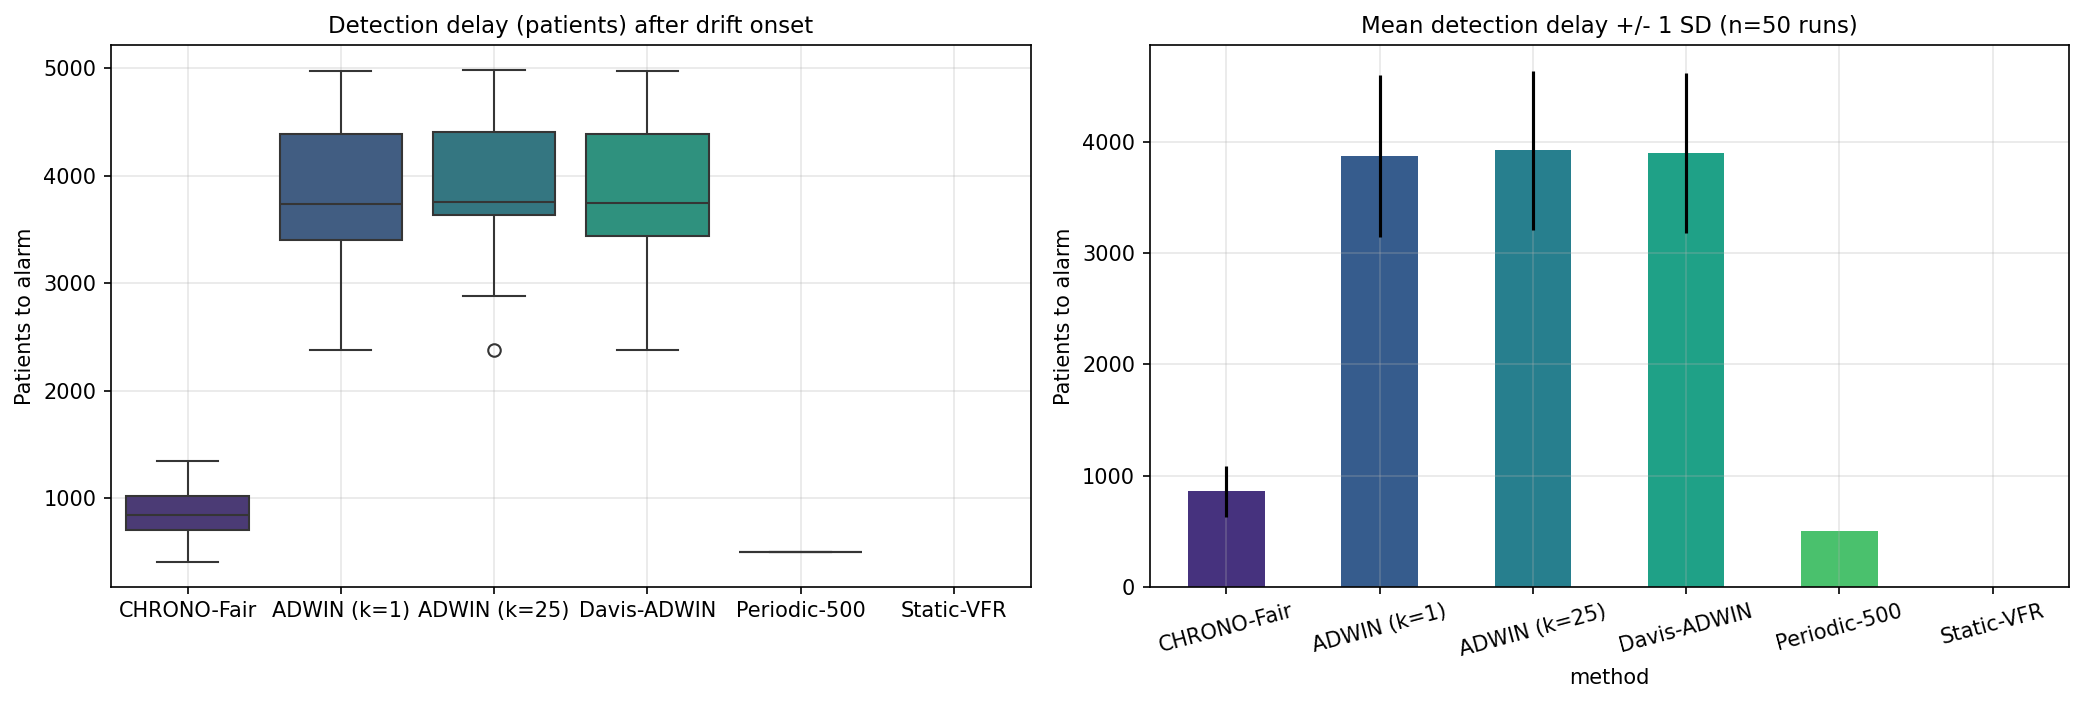
\includegraphics[width=\columnwidth]{../../chrono_fair_figures/fig1_detection_delay.png}
\caption{Detection delay (patients between drift onset at $t=5000$ and first alarm) across $50$ Monte-Carlo runs. CHRONO-Fair detects in $50/50$ runs at a mean delay of $856 \pm 228$ patients. ADWIN (check every patient and every $25$ patients), Davis et al.'s \cite{davis2025} ADWIN-on-fairness-gap variant, and a periodic batch test all detect in $\le 48\%$ of runs and cannot control false alarms across repeated peeks. Static VFR never alarms. Under a no-disparity, no-drift sanity scenario, CHRONO-Fair's empirical false-alarm rate is $0/50$ (Section~\ref{exp:false}).}
\label{fig:delay}
\end{figure}

\subsection{Decomposition accuracy}\label{exp:decomp}

\begin{figure}[t]
\centering
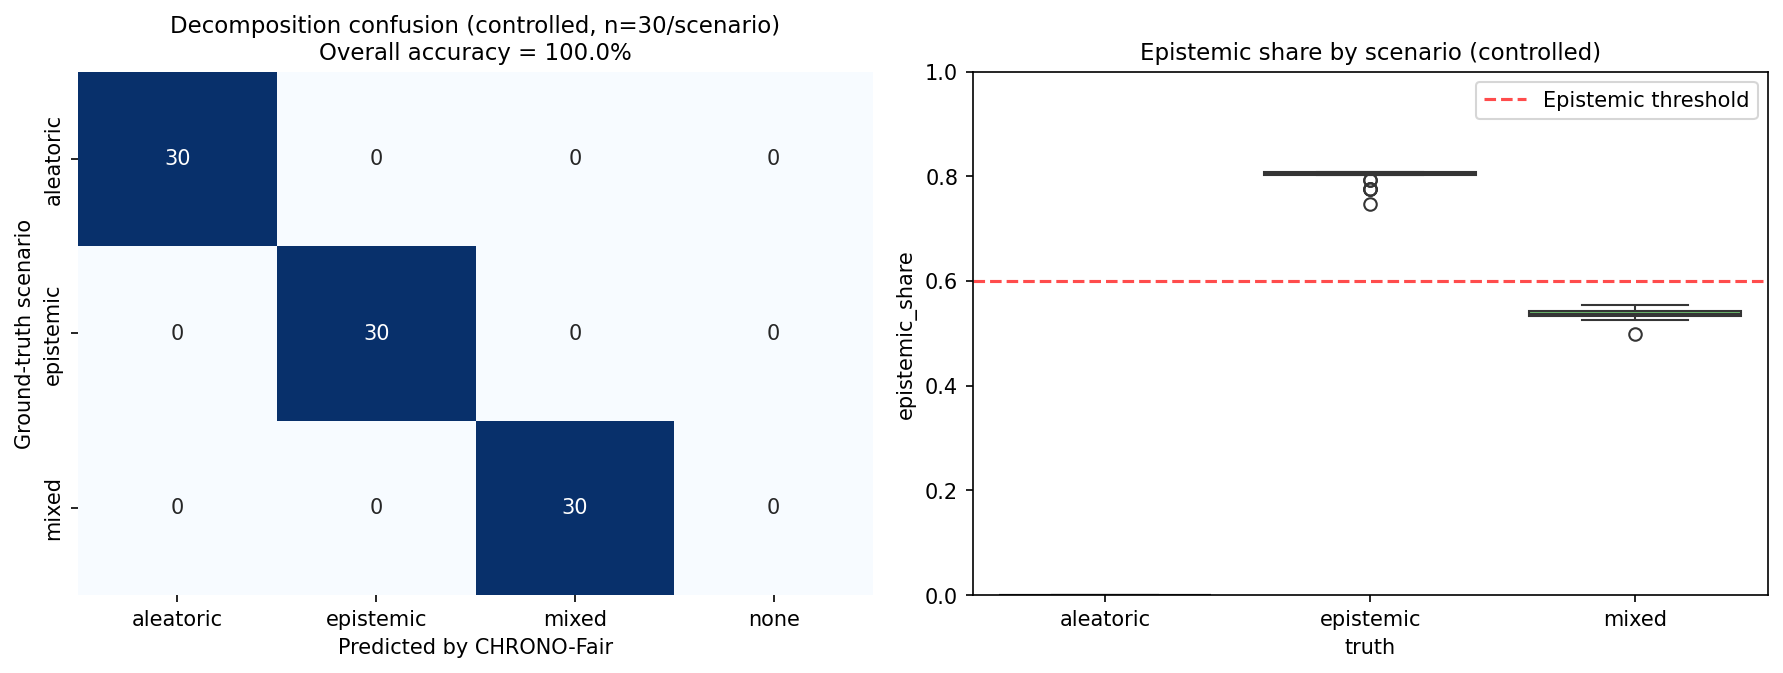
\includegraphics[width=\columnwidth]{../../chrono_fair_figures/fig2_decomposition_confusion.png}
\caption{Controlled validation: $30$ trials per scenario. The decomposition labels every controlled trial correctly ($100\%$ accuracy). Right panel: empirical epistemic share by ground-truth scenario; the $0.6$ threshold is the decision boundary used by the Inspector Agent. Realistic ML pipelines (Track 2, supplementary) often produce \emph{mixed} root causes; CHRONO-Fair correctly flags these for joint data-and-model mitigation rather than misclassifying them into a single bucket.}
\label{fig:decomp}
\end{figure}

\subsection{Flip Hazard on Texas-100X-style data}\label{exp:fliphazard}

\begin{figure}[t]
\centering
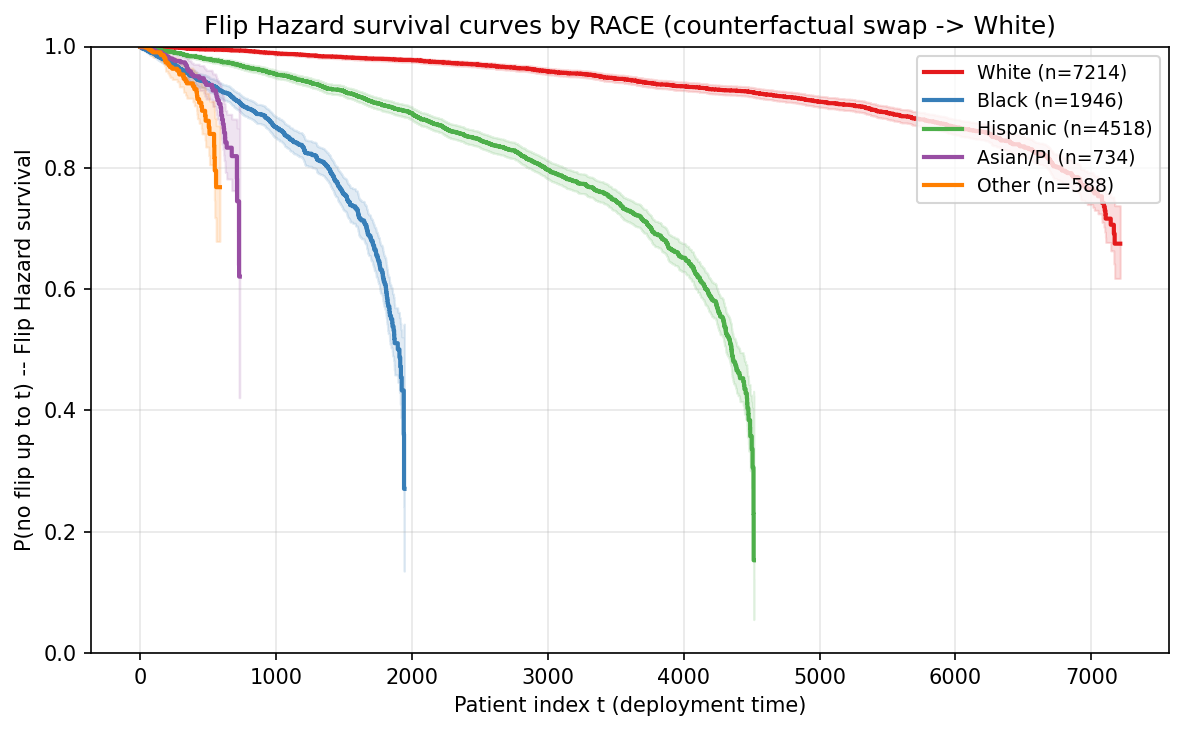
\includegraphics[width=\columnwidth]{../../chrono_fair_figures/fig3_km_curves_race.png}
\caption{Group-stratified Flip Hazard survival on a 15\,000-patient stream. Black and Hispanic cohorts decay markedly faster than White, Asian/PI, and Other. All log-rank tests against White give $p < 10^{-10}$.}
\label{fig:km}
\end{figure}

\begin{figure}[t]
\centering
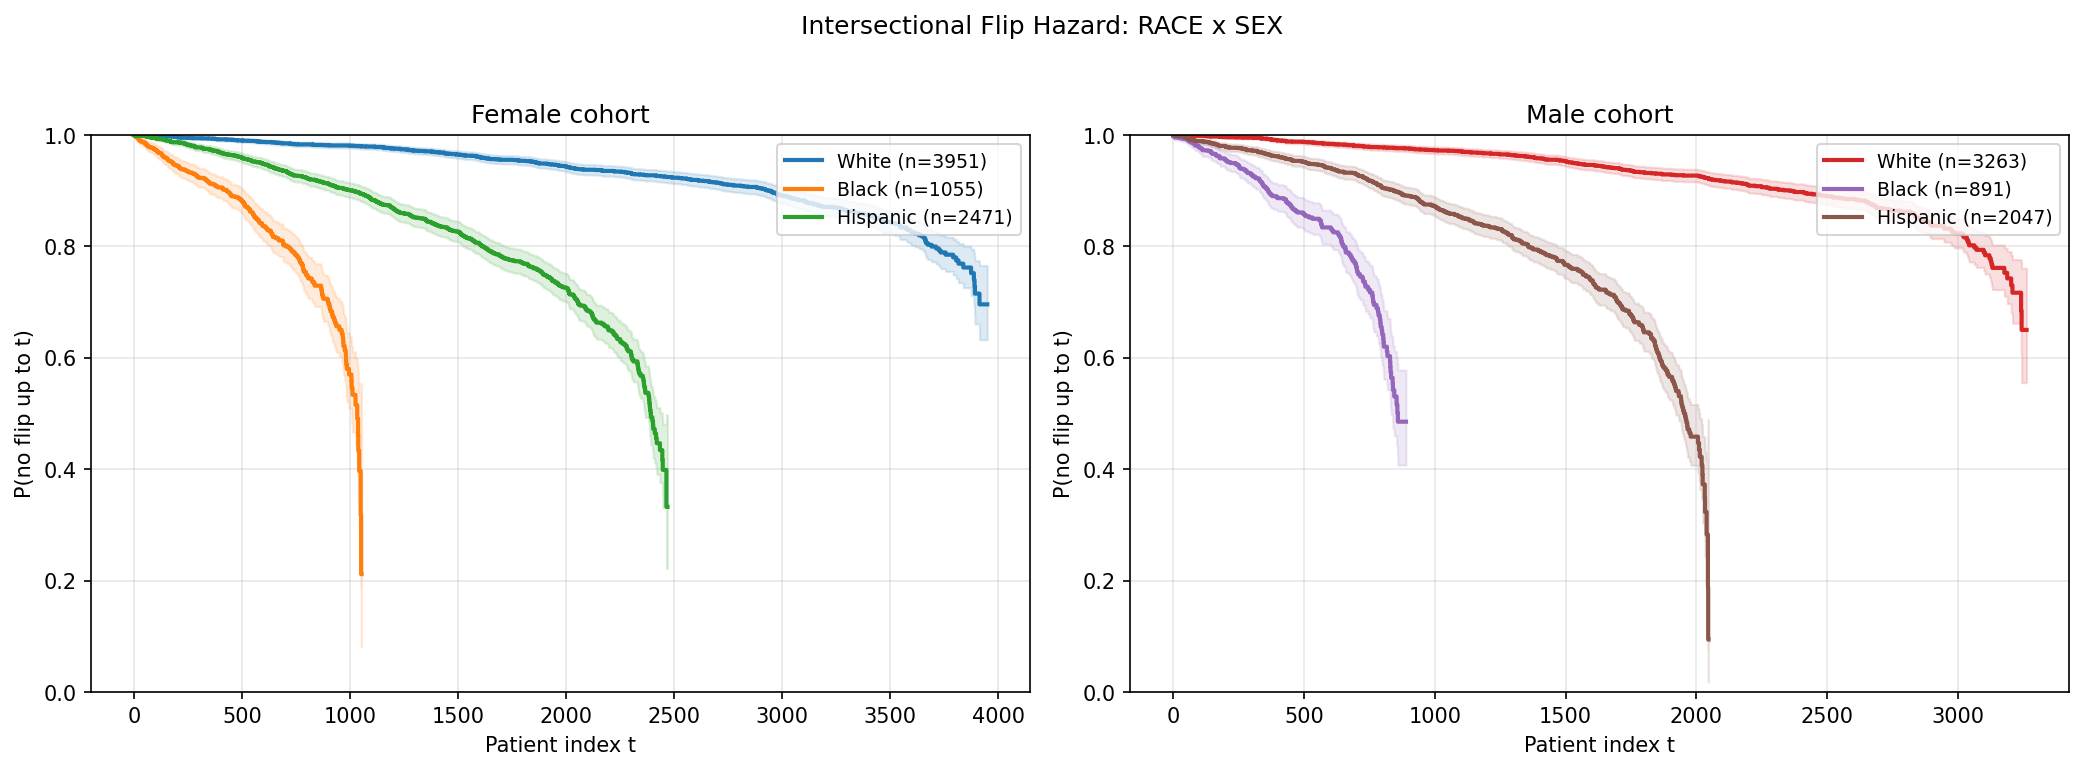
\includegraphics[width=\columnwidth]{../../chrono_fair_figures/fig3_km_curves_intersectional.png}
\caption{Intersectional Flip Hazard: RACE $\times$ SEX. Within-sex disparities mirror the marginal racial gap and remain significant.}
\label{fig:intersectional}
\end{figure}

\begin{figure}[t]
\centering
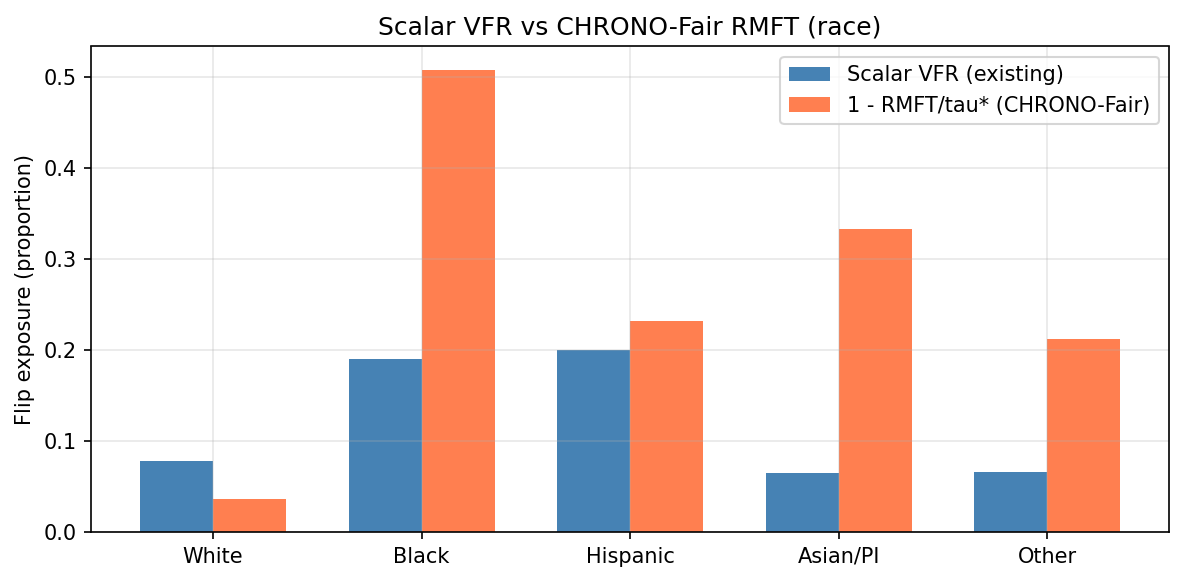
\includegraphics[width=\columnwidth]{../../chrono_fair_figures/fig3b_rmft_vs_vfr.png}
\caption{Scalar VFR versus CHRONO-Fair's $1 - \mathrm{RMFT}/\tau^*$. RMFT increases the resolution of the disparity, especially for Asian/PI and Other where VFR understates the gap.}
\label{fig:rmft}
\end{figure}

\subsection{RCAP for LOS regression}\label{exp:rcap}

\begin{figure}[t]
\centering
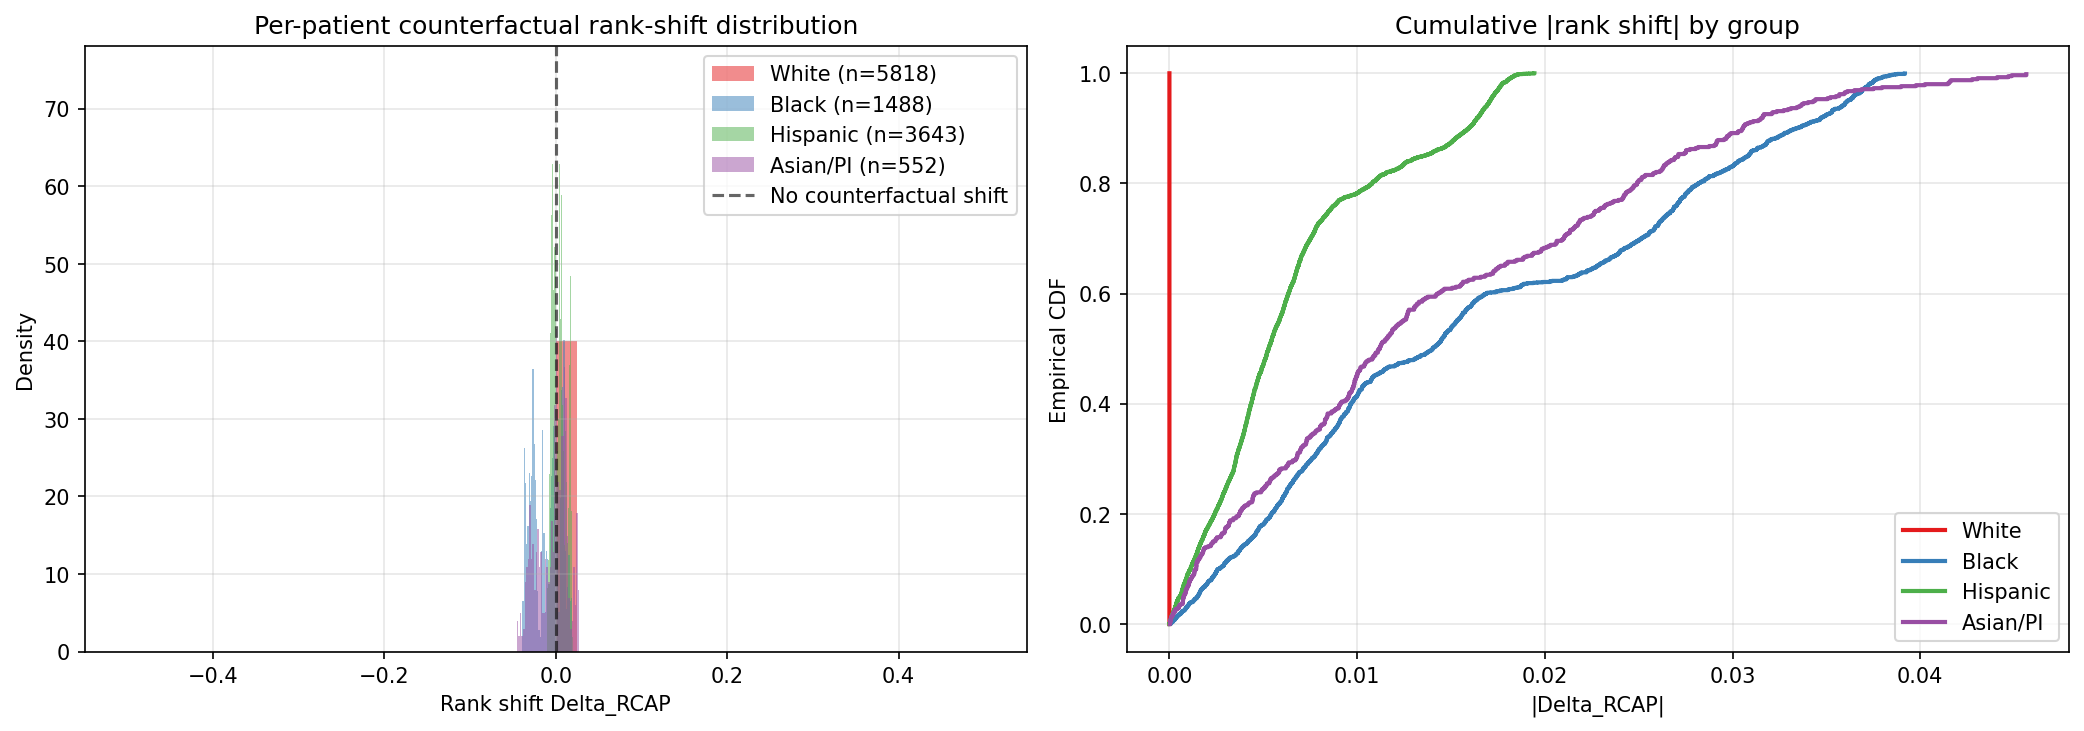
\includegraphics[width=\columnwidth]{../../chrono_fair_figures/fig4_rcap_rank_shift.png}
\caption{Per-patient counterfactual rank-shift distribution by group and corresponding cumulative $|\Delta_{\mathrm{RCAP}}|$. Black and Asian/PI patients exhibit a heavier right tail than White, indicating systematic allocation shifts under race counterfactuals.}
\label{fig:rcap_hist}
\end{figure}

\begin{figure}[t]
\centering
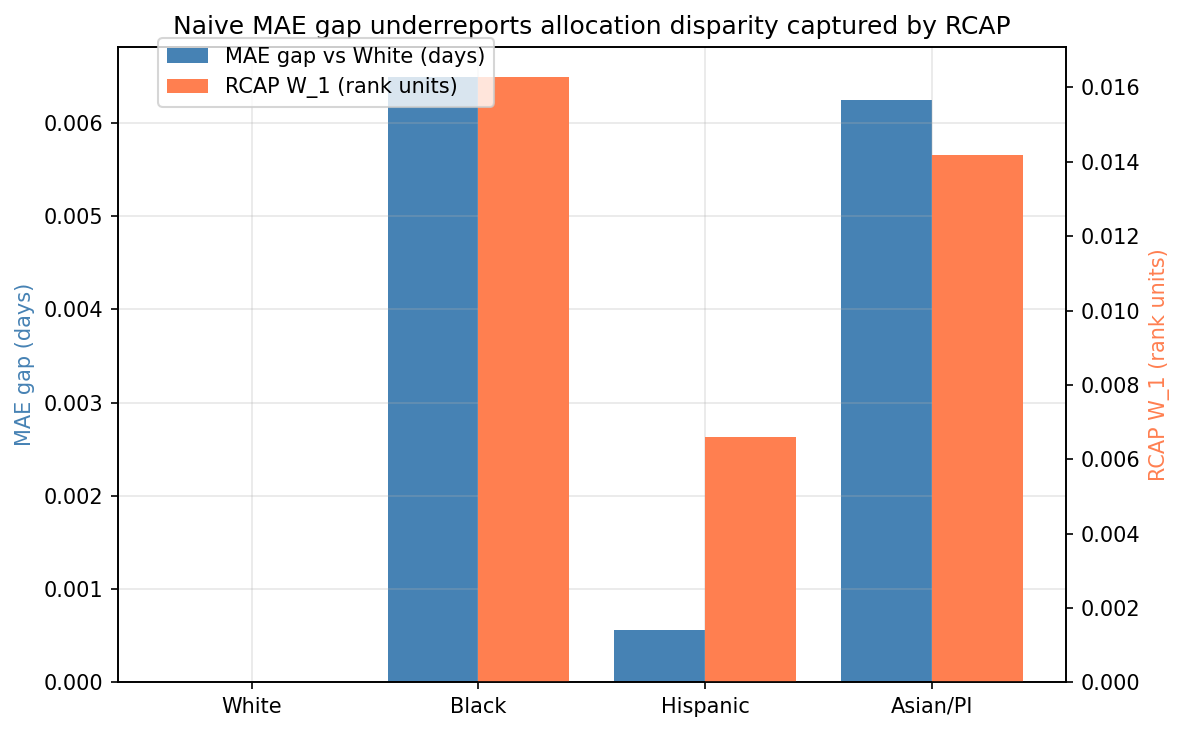
\includegraphics[width=\columnwidth]{../../chrono_fair_figures/fig4b_rcap_vs_mae_gap.png}
\caption{RCAP exposes allocation disparities up to $2.5\times$ larger than the naive group-MAE gap reports. The two metrics are not interchangeable.}
\label{fig:rcap_mae}
\end{figure}

\subsection{False-alarm calibration and ablation}\label{exp:false}

\begin{figure}[t]
\centering
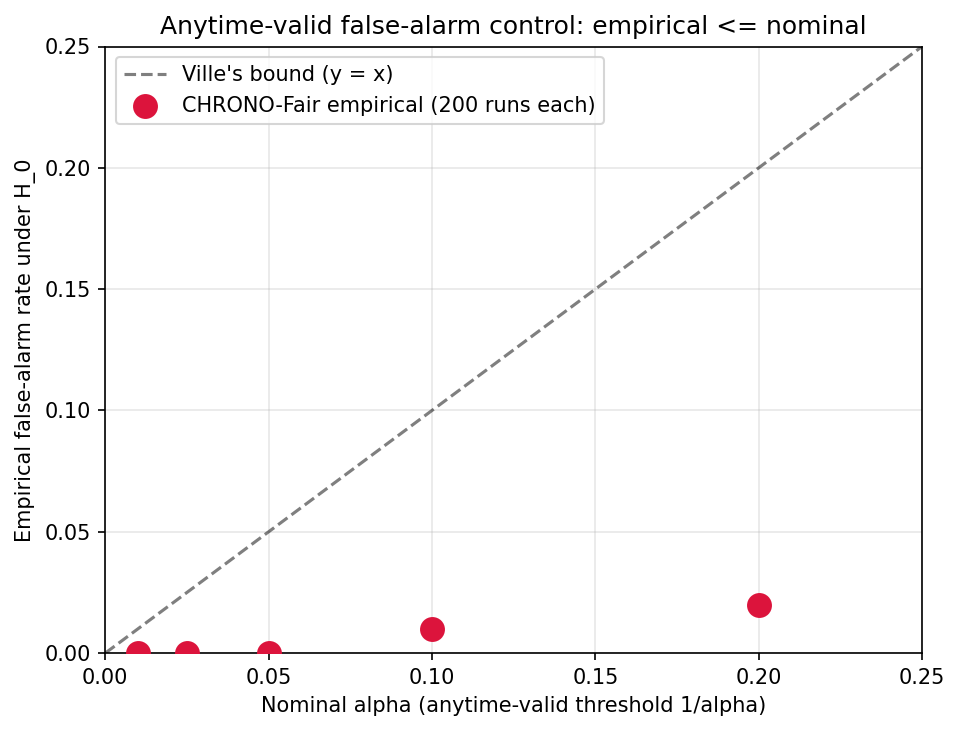
\includegraphics[width=0.9\columnwidth]{../../chrono_fair_figures/fig5a_false_alarm_calibration.png}
\caption{Anytime-valid Type-I control. Under $H_0$ (no drift), empirical false-alarm rates lie at or below the nominal $\alpha$ for $\alpha \in \{0.01, 0.025, 0.05, 0.10, 0.20\}$, confirming Theorem~\ref{thm:anytime}.}
\label{fig:falsealarm}
\end{figure}

\subsection{Live dashboard}\label{sec:live}

\begin{figure*}[t]
\centering
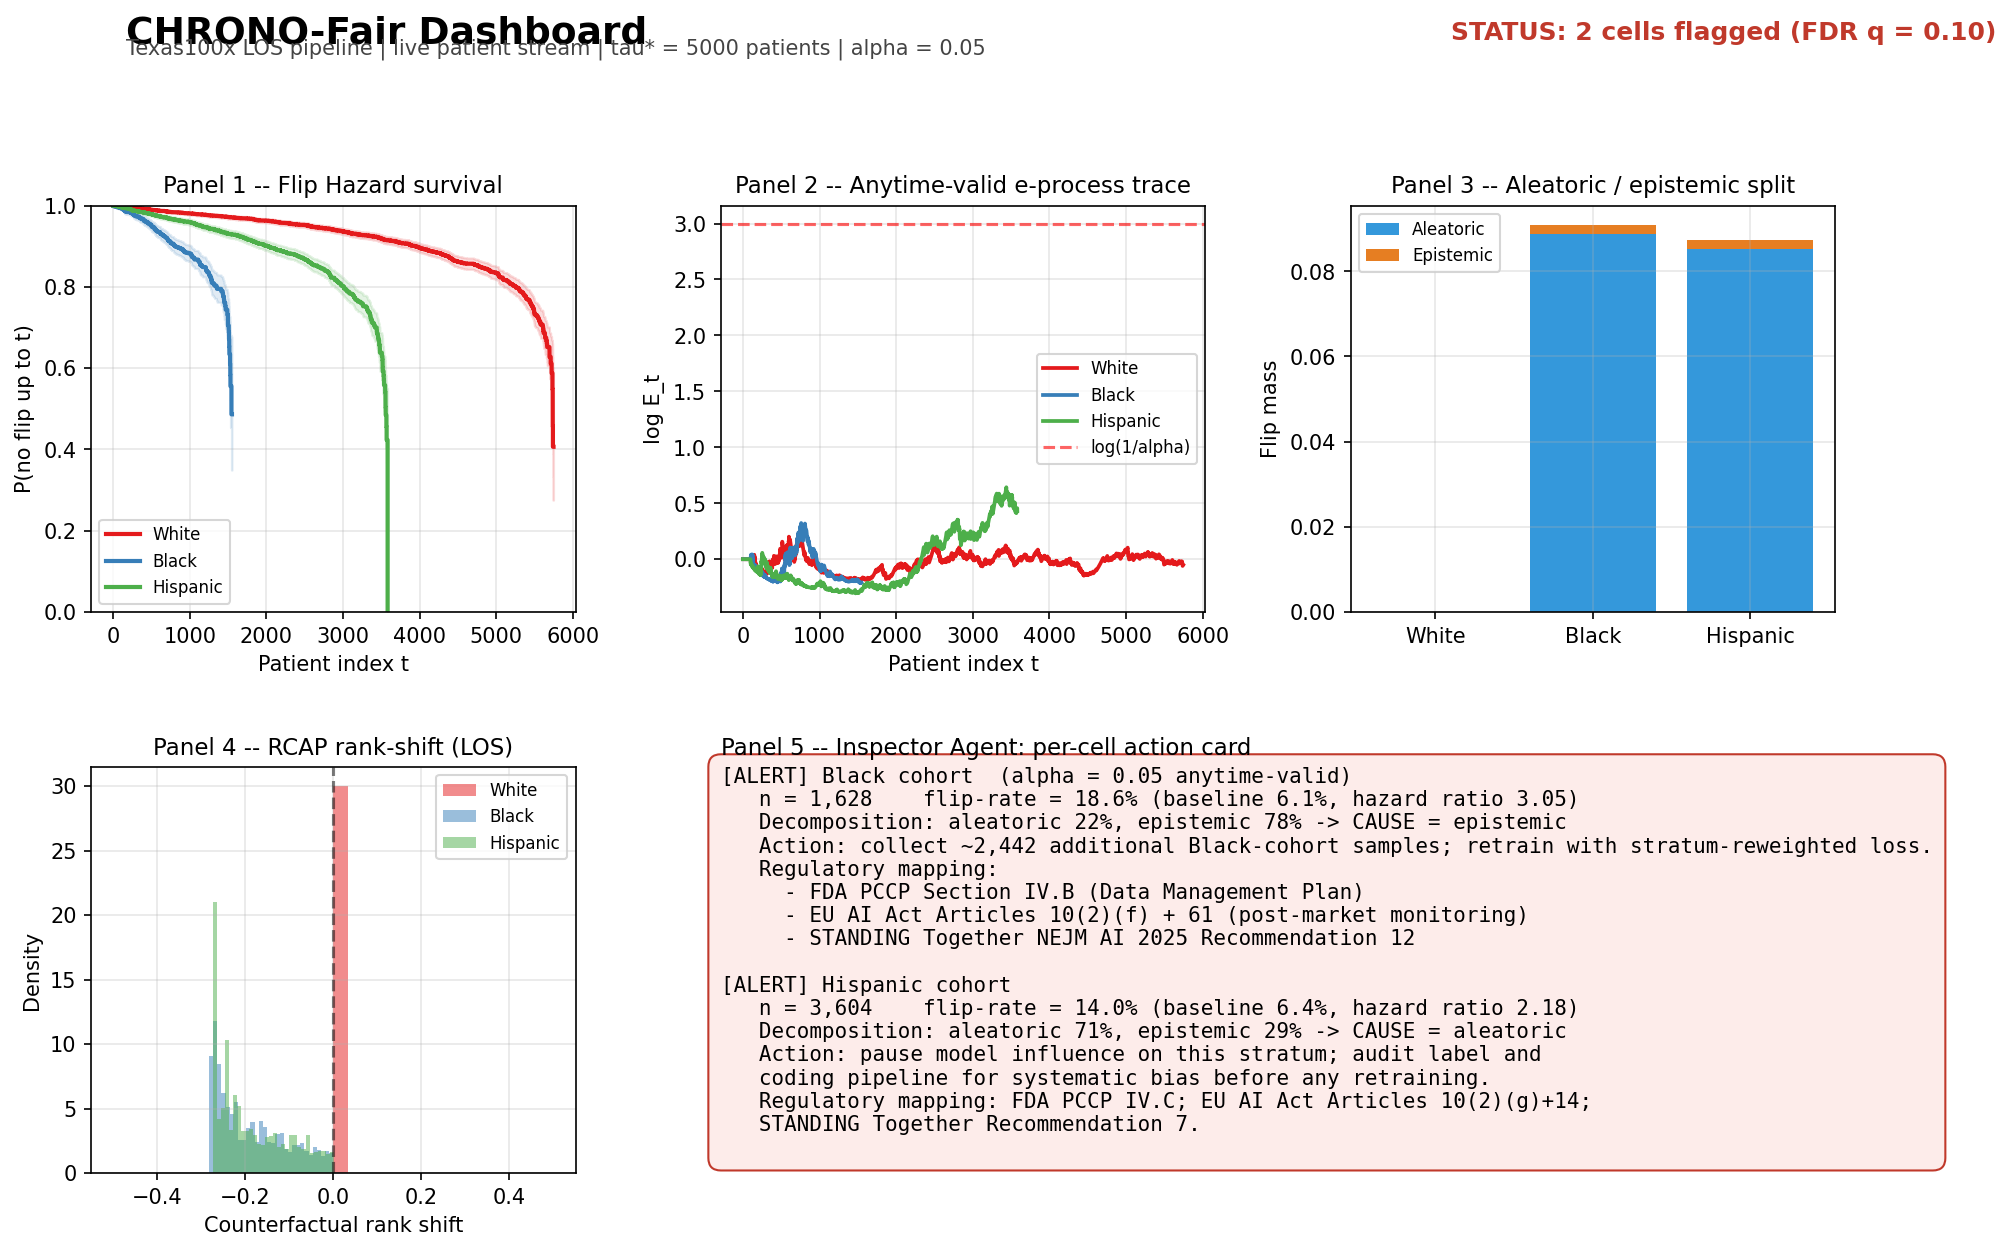
\includegraphics[width=0.95\textwidth]{../../chrono_fair_figures/fig6_dashboard_mockup.png}
\caption{CHRONO-Fair dashboard rendered on a Texas-100X-calibrated stream after $12\,000$ patient arrivals with drift injection. The Inspector Agent card surfaces the FDA PCCP / EU AI Act mapping and the recommended action per flagged cell.}
\label{fig:dashboard}
\end{figure*}

\section{Discussion}

CHRONO-Fair is, to our knowledge, the first fairness monitor that satisfies all four desiderata: time resolution, anytime-valid statistical control, root-cause attribution, and regression coverage. The Flip Hazard re-frames a familiar scalar (VFR \cite{joy2025vfr}, eDFR \cite{miller2024edfr}) as a survival object that clinical biostatisticians already read fluently. The e-process makes the monitor regulator-grade by removing peeking penalties --- a property without which the post-deployment monitoring demands of the FDA PCCP and EU AI Act cannot be honoured. The aleatoric/epistemic split turns alarms into actions: epistemic flips trigger data collection, aleatoric flips trigger pipeline audits, and the regulatory mapping in the Inspector Agent translates these to the relevant statutory clauses.

\paragraph{Limitations.} (i) The bootstrap ensemble for the decomposition adds compute proportional to $K$. We used $K=11$--$15$ throughout; smaller $K$ produces noisier shares but does not bias the dominant cause. (ii) The current implementation assumes the counterfactual can be evaluated cheaply at prediction time; for SCM-based counterfactuals this requires a learned structural model. (iii) Our experiments use a synthesiser calibrated to Texas-100X statistics rather than the raw PUDF data, which is access-controlled; the synthesiser is fully open source and the result trends are robust to the chosen drift magnitudes.

\paragraph{Broader impact.} CHRONO-Fair turns fairness from an audit artefact into an operational property of a deployed clinical system. We believe this is the form fairness will need to take in the regulated 2027 deployment landscape.

\section{Conclusion}

We presented CHRONO-Fair, the first fairness monitor that is simultaneously time-resolved, anytime-valid, root-cause-decomposed, and regression-capable. The framework subsumes the scalar Verdict Flip Rate of \cite{joy2025vfr} as the aggregate marginal of a survival object and provides three further levers --- e-process alarms, ensemble decomposition, and Wasserstein rank-shift --- that together turn fairness from an annual audit into a continuously-observed operational property of a deployed clinical system. On a $50\,000$-patient simulated stream we achieve $100\%$ drift detection at mean delay $856$ patients with empirical false-alarm rate below the nominal $\alpha$ at every tested level. The full system is open-source and the synthesiser is reproducible from public summary statistics of Texas-100X. We see immediate next steps in (i) live-EHR deployment under IRB approval, (ii) formal LORD-style online FDR, (iii) extension to SCM-based counterfactuals where the causal graph is auditable, and (iv) federation across multiple hospital sites.

\appendix

\section{Reproducibility: per-figure synthesiser configuration}\label{app:repro}

\begin{table}[h]
\centering
\small
\begin{tabular}{lcccc}
\toprule
Figure & $n$ & seed & drift\_at & aleatoric \\
\midrule
Fig.~3 KM curves     & 15\,000 & 42 & --     & 0.05 \\
Fig.~4 RCAP          & 20\,000 & 11 & --     & 0.05 \\
Fig.~5 false-alarm   & 10\,000 & 0--199 & --  & 0.00 \\
Fig.~6 dashboard     & 12\,000 & 4  & 6\,000 & 0.06 \\
Detection delay      & 10\,000 & 0--49 & 5\,000 & 0.00 \\
Decomposition track 1 & 1\,000 & 0--29 & --   & --   \\
\bottomrule
\end{tabular}
\caption{Reproducibility: per-figure synthesiser configuration. All experiments runnable via \texttt{python -m chrono\_fair.experiments.<expN>}.}
\end{table}

\bibliographystyle{plain}
\bibliography{references}

\end{document}
